% res_steady.tex -- Results 4.1 (cont.): the steady payload error, rig and twin.
% 17 Oct (v3_full): rewritten around the measured rod pull after the appendix re-fly on the freeze tree
% (docs/analysis/appendix_refly_2026-10-17.md: C-X1, C-X2, C-D1, C-D4, C-R1-R4 confirmed; C-D2, C-D3, C-D5 falsified;
% C-G1, C-G2 unresolved; the reviewer's must-not-say list honoured: no 8.4 cm, no "learns the push" vertically, no
% 0.76 N as learned, no geometric explanation of +17.1 cm, the +13 cm box offset is not a tracking error, no "the model
% integral fails on the thrust-map error", the mass result always with the measured pull and the rigid-rod twin) and
% the exploratory cable_source model pair (R2084-R2087: push -7.95 cm, +20 % mass +22.2 cm). Rig sources unchanged:
% registry RIG-1001-*, RIG-1007-r0001/r002/r20004 (fig:rig_integral), docs/rig_2026-09-30_review.md.

\subsubsection{Steady payload error}
\label{sec:res_steady}

This part of RQ1 asks what leaves a steady error in the payload's position, and what removes it. Each source is
set against the same flight without its remedy, its baseline; the bar is the ring back within 1\,cm of its target.
On the rig, the measured rod pull is what changed the picture, and it does the same in the twin.

\paragraph{On the rig: the model integral and the measured rod pull}
\label{sec:res_rig_integral}
% Rig 7 Oct: RIG-1007-r0001 (no integral), r002 (model integral, planned pull), r20004 (model integral +
% measured pull); planner log.csv; figure tools/thesis_rig_figures.py rig_integral.

On 7 October the rig flew three hovers at 1.0\,m with four UAVs, changing one thing at a time
(Figure~\ref{fig:rig_integral}). Without an integral the ring sank in the 5\,s it held before LAND. The model
integral brought it back to its target by learning a downward force of up to 0.9\,N, but the ring then bobbed
at about 0.2\,Hz. With the trackers' measured rod pull added (Section~\ref{sec:tracker}) it held within 2\,cm
and the integral learned only 0.1\,N: most of the missing force was in the rods' pull, which the planned pull
got wrong. On the circle and the figure-eight, the measured pull with the rods planned at 60$^\circ$ cut the
standard deviation of the ring's height from 4.8--4.9 to 0.5--0.6\,cm (Table~\ref{tab:T7}). Each is one run; the
measured-pull hover held for 7\,s, ending before the first swing of the integral-only run, so the circle and the
figure-eight, flown for 36 and 68\,s, carry the claim that the swing is gone.

\begin{figure}[htbp]
\centering
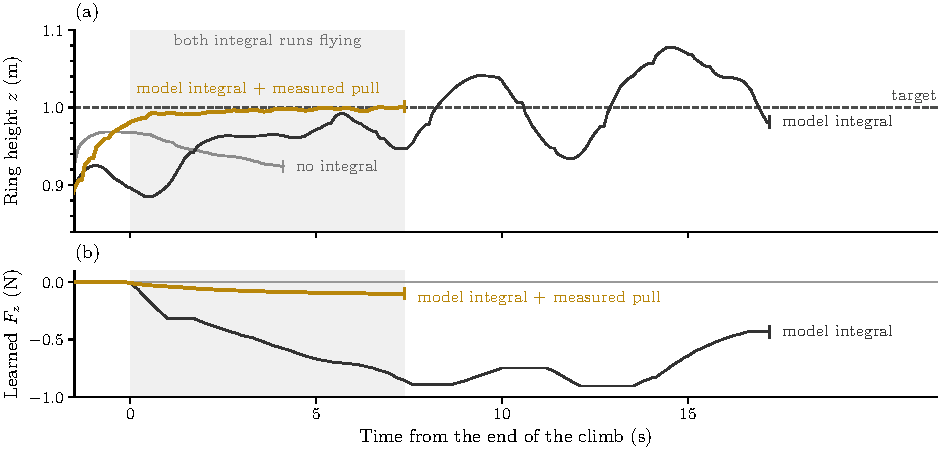
\includegraphics[width=\textwidth]{Images/rig_integral.pdf}
\caption[The model integral and the measured pull on the rig]{Ring height on the rig in a hover at 1.0\,m with
four UAVs, one change at a time (7 October, one run each; each trace ends at LAND, marked by a tick; shaded: the
7\,s both integral runs flew). (a) Without an integral the ring sank from 0.97 to 0.92\,m. With the model integral
it dipped to 0.89\,m after the climb, came back up, and from 8\,s bobbed between 0.93 and 1.08\,m at about
0.2\,Hz. With the integral and the trackers using the measured rod pull it held between 0.98 and 1.00\,m.
(b) The vertical force the model integral learned (negative: downward, a force the model lacked): up to
$-0.9$\,N with the planned pull, $-0.1$\,N with the measured one. The flat stretches are the integral frozen by
design while the ring moves faster than 0.05\,m/s vertically.}
\label{fig:rig_integral}
\end{figure}

\paragraph{External forces}
\label{sec:res_force}

In the twin a constant force was applied to the hovering ring for 15\,s: 0.6\,N downward, about the weight of a
60\,g object, and 0.4\,N horizontally (Table~\ref{tab:disturbance}). The two axes now behave differently. The
vertical push leaves no steady offset, with or without an integral: each tracker's measured pull takes up its share
within about a second, so the ring dips 1.4\,cm and is back within 1\,cm 1.0--1.1\,s after the onset, and the
integral is left with nothing to remove. An exploratory pair with the trackers on the planner's pull instead, and
nothing else changed, left the ring 8.0\,cm low under the same push, which places the effect in the measured pull.
Horizontally the measured pull does not act on the ring's position, and the push leaves the ring 4.8\,cm off its
target; the model integral removes that offset, its force settling at 0.32\,N against the 0.40\,N applied
(Figure~\ref{fig:disturbance}). It does so as integral action does: the peak is barely reduced, because the integral
($1/k_i = 2.5$\,s) is slower than the cascade, and when the push ends the integral still holds its force and drives
the ring past the target by about as much as the push displaced it at onset (5.3\,cm). Doubling $k_i$, or keeping
the integral's speed gate only for the first 5\,s after the lift, made no difference the resolution rule could
resolve on the vertical push (Table~\ref{tab:gain}, Appendix~\ref{sec:app_tests}); there the integral barely moves.
When one UAV produces more thrust than its map assumes, neither form of the integral leaves a height or horizontal
error, and the ring hovers level (0.1$^\circ$); the trace reads as that UAV's own measured pull taking up its error,
which a force on the payload could not represent, though no one-variable pair separates it.

\begin{figure}[htbp]
\centering
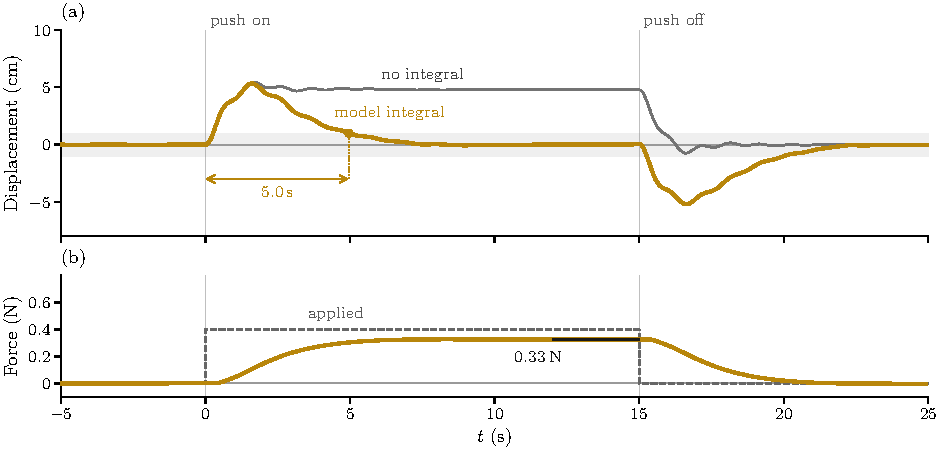
\includegraphics[width=\textwidth]{Images/disturbance.pdf}
\caption[Rejection of a horizontal force on the ring]{Rejection of a constant horizontal force on the ring in the
rig twin: three carriers, hover at 1.0\,m, the measured rod pull; a 0.4\,N push acts from 0 to 15\,s; one run of
each case (Table~\ref{tab:disturbance} gives both runs and the vertical push). (a) Ring displacement along the push,
relative to its mean over the 5\,s before: no integral (grey) and the integral in the planner's model (gold). Band:
$\pm 1$\,cm. Arrow: the time for the model integral to bring the ring back within 1\,cm for good. (b) Change of the
model integral's force $\mathbf{d}$ along the push from its value before the push (gold), against the applied force
(dashed). Black bar: its mean over the last 3\,s of the push.}
\label{fig:disturbance}
\end{figure}

\begin{table}[htbp]
\centering
\caption[Disturbance rejection in the twin]{Disturbance rejection in the rig twin: three carriers in hover at 1.0\,m,
$\epsilon = 0$, two runs per cell on the freeze code tree. Displacement along the force, relative to its mean over
the 5\,s before the push; time to within 1\,cm after the onset; the change of the integral's force from its value
before the push.}
\label{tab:disturbance}
% generated by tools/thesis_sim_tables.py on the freeze tree (17 Oct; appendix re-fly R2027-R2033, R2039-R2045), then
% edited by hand: the planned-pull column (exploratory pair R2084, R2086, cable_source model) and footnotes a-c from
% the reviewer's corrections (docs/analysis/appendix_refly_2026-10-17.md).
\footnotesize
\setlength{\tabcolsep}{4pt}
\begin{tabular}{lcccc}
\toprule
 & \multicolumn{3}{c}{Measured rod pull} & Planned pull \\
\cmidrule(lr){2-4}\cmidrule(lr){5-5}
 & No integral & Target shift & Model integral & No integral$^c$ \\
\midrule
\multicolumn{5}{l}{\emph{0.6\,N downward push on the ring}} \\
\quad steady displacement (cm) & 0.0 (2) & 0.0 (2) & 0.0 (2) & 8.0 (2) \\
\quad peak displacement (cm) & 1.4 (2) & 1.3 (2) & 1.3 (2) & -- \\
\quad overshoot after release (cm) & 1.4 (2) & 1.5 (2) & 1.4 (2) & -- \\
\quad time to within 1\,cm (s) & 1.1 (2) & 1.0 (2) & 1.1 (2) & -- \\
\quad change of the integral force (N) & -- & -- & 0.10$^a$ (2) & -- \\
\midrule
\multicolumn{5}{l}{\emph{0.4\,N horizontal push on the ring}} \\
\quad steady displacement (cm) & 4.8 (2) & n/a & 0.0 (2) & -- \\
\quad peak displacement (cm) & 5.4 (2) & n/a & 5.5 (2) & -- \\
\quad overshoot after release (cm) & 0.7 (2) & n/a & 5.3 (2) & -- \\
\quad time to within 1\,cm (s) & -- & n/a & 4.9 (2) & -- \\
\quad change of the integral force (N) & -- & n/a & 0.32 (2) & -- \\
\midrule
\multicolumn{5}{l}{\emph{One UAV producing more thrust than its map assumes$^b$}} \\
\quad height error (cm) & -- & 0.0 (2) & $-$0.1 (2) & -- \\
\quad horizontal error (cm) & -- & 0.0 (2) & 0.0 (2) & -- \\
\quad ring tilt (\si{\degree}) & -- & 0.1 (2) & 0.1 (2) & -- \\
\bottomrule
\multicolumn{5}{p{0.95\textwidth}}{\footnotesize $^a$\,Not a learned force: it doubles with the integral gain
(0.21--0.22\,N at $k_i = 0.8$) and drifts by $-0.05$\,N with no push; the measured pull has already taken the push
up. $^b$\,Its real throttle offset 0.03 below the 0.185 its tracker assumes. $^c$\,Exploratory pair: the trackers on
the planner's pull, everything else as the first column, flown on a later code tree whose flight code differs only by
switches that are off.}
\end{tabular}

\end{table}

\paragraph{Wrong model values}
\label{sec:sim_robustness}

The controller is given the payload's mass, the rod lengths, the attachment radius and each UAV's thrust map; on the
rig each is measured, and each can be wrong. In the twin's hover with one wrong value in the controller while the
simulated rig keeps the true ones (Table~\ref{tab:robust}, Appendix~\ref{sec:app_robust}), a payload mass typed
20\,\% high or low leaves the hover where it was, with or without the integral, because the measured pull at each UAV
carries what the ring actually weighs; in an exploratory pair on the planner's pull the same $+20$\,\% error left the
ring 22.2\,cm high. That is a result of the rigid-rod twin on the measured pull, not a licence to type the mass
loosely. Rods typed 5\,cm long are absorbed when they are measured at the hand-over; unmeasured, they leave the ring
17.1\,cm high with or without the integral, whose tautness gate stays closed because the rods read as partly slack.
An attachment radius typed 2\,cm large leaves the ring 0.9\,cm high, and the vertical integral winds up through the
hold without moving it, to 0.76\,N by LAND: not a learned force, and a reason the integral's bound and its warning
matter. All 28 flights landed, and the ring's tilt stayed at 0.1$^\circ$.

\paragraph{The tracker's initial condition}
\label{sec:res_ic}

An earlier version of the tracker relaxed its initial condition to a box with $\epsilon = 0.025$
(Section~\ref{sec:tracker}). On the freeze tree the box holds the ring 13.1\,cm above its target in hover and
13.0\,cm on the orbit, where pinning node~0 to the measurement holds it within 0.1\,cm, and pinning also cuts the
orbit's horizontal error from 3.9 to 0.7\,cm (Table~\ref{tab:x0}, Appendix~\ref{sec:app_tests}). The offset is not
a tracking error of the UAVs: the references the planner sends them are themselves 10.6\,cm higher. It is a bias in
the cascade, not a force, which is why no force estimate of the earlier stack could find it.

\paragraph{The breakaway cap}
\label{sec:res_cap}

On the rig on 1 October (Table~\ref{tab:rig_oct1}, Appendix~\ref{sec:app_rig}), without the height integral the ring
held 5\,cm low at 0.5\,m, and at higher targets it sat 20--30\,cm low before the integral took over, which then
saturated at its bound. The cause was found afterwards in the logs: the breakaway freeze of
Section~\ref{sec:takeoff} had held the pull at the fraction reached at breakaway for the whole flight, so the trackers
were told the rods pull 7--27\,\% less than they do. Holding the pull at 75\,\% in the twin reproduced the rig's
height shortfall and its steeper rods. The cap has been released once the lift starts since 7 October.

\paragraph{The rig's pull towards $-x$.} In every rig flight of 1 October the ring sat 3--17\,cm from its horizontal
reference, always towards the room's $-x$ direction, and nothing in the controller then pulled it back. The offset
kept its direction when the whole system was rotated by 124$^\circ$, so it does not come from a particular UAV, rod
or the ring. Estimated offline from the UAVs' delivered thrust less the total weight, the force behind it was
0.41--0.52\,N towards $-x$, about 1$^\circ$ of the fleet's thrust; moving the system 1.1\,m towards $+x$ reduced the
offset to 3--5\,cm, in a single flight. A motion-capture ground plane tilted by about 1$^\circ$, or air moving in
the room, remain the two explanations; the model integral, which removes a horizontal force in the twin, has flown on
the rig since 7 October.

\paragraph{Tilt and height.} On the rig the ring's mean tilt fell from 5.0$^\circ$ at 0.45\,m to 1.6$^\circ$ at
0.94\,m (1 October): close to the floor the ring sits in the UAVs' downwash and its recirculation, and flying higher
was the most effective single change for a steady ring.

\paragraph{Sources of steady error}

Table~\ref{tab:error_sources} collects the sources found, how each shows at the payload and what removes it. The
approaches to model error flown on the earlier stack (a force balance, an offset-free observer, the measured cable
force, a thrust-gain trim, the rods' mass in the planner) are recorded in Appendix~\ref{sec:app_methods}; the measured
cable force is the one that became the default.

\begin{table}[htbp]
\centering
\footnotesize
\caption{Sources of steady payload error found in this work, how each shows at the payload and what
removes it, on the current controller.}
\label{tab:error_sources}
\begin{tabularx}{\textwidth}{>{\raggedright\arraybackslash}p{3.2cm}>{\raggedright\arraybackslash}X>{\raggedright\arraybackslash}Xl}
\toprule
Source & Signature at the payload & Remedy & Section \\
\midrule
Tracker's relaxed initial condition & held high in hover and on the orbit (13\,cm in the twin); in the
references, not a tracking error; not a force & pin node~0 to the measurement & \ref{sec:res_ic} \\ \addlinespace
Breakaway cap held for the whole flight & held low; rods steeper than planned (rig) & release the cap once
the lift starts & \ref{sec:res_cap} \\ \addlinespace
A vertical force on the ring & none on the measured pull; on the planned pull a steady drop (8\,cm for 0.6\,N,
exploratory) & the measured rod pull at each UAV & \ref{sec:res_force} \\ \addlinespace
A horizontal force (a push, wind, the rig's pull towards $-x$) & steady displacement along the force (4.8\,cm for
0.4\,N in the twin) & the model integral & \ref{sec:res_force} \\ \addlinespace
Payload mass typed wrong & none on the measured pull in the rigid-rod twin; on the planned pull a height offset
(22\,cm for $+20$\,\%, exploratory) & the measured rod pull & \ref{sec:sim_robustness} \\ \addlinespace
Rods typed long, not measured & held high (17\,cm for $+5$\,cm); the rods read partly slack, so the integral's gate
stays closed & measure the rods at the hand-over & \ref{sec:sim_robustness} \\ \addlinespace
Attachment radius typed wrong & held 0.9\,cm high for $+2$\,cm; the vertical integral winds up without effect &
none yet: the radius is measured on the rig & \ref{sec:sim_robustness} \\ \addlinespace
One UAV's thrust map wrong & none in hover on the measured pull; a tilt and a horizontal offset on the planned
pull (earlier stack) & that UAV's own measured pull & \ref{sec:res_force} \\
\bottomrule
\end{tabularx}
\end{table}

\paragraph{Answer to RQ1, steady errors.} The measured rod pull, not the integral, is what holds the ring's height on
this controller: in the rigid-rod twin it takes up a vertical push and an error in the typed payload mass at the UAVs
themselves (separated from the other changes by an exploratory one-variable pair) and, on the trace, one UAV's
thrust-map error; on the rig it removed most of the force the integral had been learning.
The model integral is left with horizontal forces, which it removes, and its vertical part can wind up on an error it
cannot see. The two sources that are not forces, the tracker's relaxed initial condition and the breakaway cap, are
removed at their source, and rods typed long must be measured at the hand-over.
